% Generated by Sphinx.
\def\sphinxdocclass{report}
\documentclass[letterpaper,10pt,english]{sphinxmanual}
\usepackage[utf8]{inputenc}
\DeclareUnicodeCharacter{00A0}{\nobreakspace}
\usepackage[T1]{fontenc}
\usepackage{babel}
\usepackage{times}
\usepackage[Bjarne]{fncychap}
\usepackage{longtable}
\usepackage{sphinx}
\usepackage{multirow}


\title{Strombolian Eruption Simulation Documentation}
\date{December 13, 2012}
\release{0.1}
\author{Jay Laura}
\newcommand{\sphinxlogo}{}
\renewcommand{\releasename}{Release}
\makeindex

\makeatletter
\def\PYG@reset{\let\PYG@it=\relax \let\PYG@bf=\relax%
    \let\PYG@ul=\relax \let\PYG@tc=\relax%
    \let\PYG@bc=\relax \let\PYG@ff=\relax}
\def\PYG@tok#1{\csname PYG@tok@#1\endcsname}
\def\PYG@toks#1+{\ifx\relax#1\empty\else%
    \PYG@tok{#1}\expandafter\PYG@toks\fi}
\def\PYG@do#1{\PYG@bc{\PYG@tc{\PYG@ul{%
    \PYG@it{\PYG@bf{\PYG@ff{#1}}}}}}}
\def\PYG#1#2{\PYG@reset\PYG@toks#1+\relax+\PYG@do{#2}}

\expandafter\def\csname PYG@tok@gd\endcsname{\def\PYG@tc##1{\textcolor[rgb]{0.63,0.00,0.00}{##1}}}
\expandafter\def\csname PYG@tok@gu\endcsname{\let\PYG@bf=\textbf\def\PYG@tc##1{\textcolor[rgb]{0.50,0.00,0.50}{##1}}}
\expandafter\def\csname PYG@tok@gt\endcsname{\def\PYG@tc##1{\textcolor[rgb]{0.00,0.25,0.82}{##1}}}
\expandafter\def\csname PYG@tok@gs\endcsname{\let\PYG@bf=\textbf}
\expandafter\def\csname PYG@tok@gr\endcsname{\def\PYG@tc##1{\textcolor[rgb]{1.00,0.00,0.00}{##1}}}
\expandafter\def\csname PYG@tok@cm\endcsname{\let\PYG@it=\textit\def\PYG@tc##1{\textcolor[rgb]{0.25,0.50,0.56}{##1}}}
\expandafter\def\csname PYG@tok@vg\endcsname{\def\PYG@tc##1{\textcolor[rgb]{0.73,0.38,0.84}{##1}}}
\expandafter\def\csname PYG@tok@m\endcsname{\def\PYG@tc##1{\textcolor[rgb]{0.13,0.50,0.31}{##1}}}
\expandafter\def\csname PYG@tok@mh\endcsname{\def\PYG@tc##1{\textcolor[rgb]{0.13,0.50,0.31}{##1}}}
\expandafter\def\csname PYG@tok@cs\endcsname{\def\PYG@tc##1{\textcolor[rgb]{0.25,0.50,0.56}{##1}}\def\PYG@bc##1{\setlength{\fboxsep}{0pt}\colorbox[rgb]{1.00,0.94,0.94}{\strut ##1}}}
\expandafter\def\csname PYG@tok@ge\endcsname{\let\PYG@it=\textit}
\expandafter\def\csname PYG@tok@vc\endcsname{\def\PYG@tc##1{\textcolor[rgb]{0.73,0.38,0.84}{##1}}}
\expandafter\def\csname PYG@tok@il\endcsname{\def\PYG@tc##1{\textcolor[rgb]{0.13,0.50,0.31}{##1}}}
\expandafter\def\csname PYG@tok@go\endcsname{\def\PYG@tc##1{\textcolor[rgb]{0.19,0.19,0.19}{##1}}}
\expandafter\def\csname PYG@tok@cp\endcsname{\def\PYG@tc##1{\textcolor[rgb]{0.00,0.44,0.13}{##1}}}
\expandafter\def\csname PYG@tok@gi\endcsname{\def\PYG@tc##1{\textcolor[rgb]{0.00,0.63,0.00}{##1}}}
\expandafter\def\csname PYG@tok@gh\endcsname{\let\PYG@bf=\textbf\def\PYG@tc##1{\textcolor[rgb]{0.00,0.00,0.50}{##1}}}
\expandafter\def\csname PYG@tok@ni\endcsname{\let\PYG@bf=\textbf\def\PYG@tc##1{\textcolor[rgb]{0.84,0.33,0.22}{##1}}}
\expandafter\def\csname PYG@tok@nl\endcsname{\let\PYG@bf=\textbf\def\PYG@tc##1{\textcolor[rgb]{0.00,0.13,0.44}{##1}}}
\expandafter\def\csname PYG@tok@nn\endcsname{\let\PYG@bf=\textbf\def\PYG@tc##1{\textcolor[rgb]{0.05,0.52,0.71}{##1}}}
\expandafter\def\csname PYG@tok@no\endcsname{\def\PYG@tc##1{\textcolor[rgb]{0.38,0.68,0.84}{##1}}}
\expandafter\def\csname PYG@tok@na\endcsname{\def\PYG@tc##1{\textcolor[rgb]{0.25,0.44,0.63}{##1}}}
\expandafter\def\csname PYG@tok@nb\endcsname{\def\PYG@tc##1{\textcolor[rgb]{0.00,0.44,0.13}{##1}}}
\expandafter\def\csname PYG@tok@nc\endcsname{\let\PYG@bf=\textbf\def\PYG@tc##1{\textcolor[rgb]{0.05,0.52,0.71}{##1}}}
\expandafter\def\csname PYG@tok@nd\endcsname{\let\PYG@bf=\textbf\def\PYG@tc##1{\textcolor[rgb]{0.33,0.33,0.33}{##1}}}
\expandafter\def\csname PYG@tok@ne\endcsname{\def\PYG@tc##1{\textcolor[rgb]{0.00,0.44,0.13}{##1}}}
\expandafter\def\csname PYG@tok@nf\endcsname{\def\PYG@tc##1{\textcolor[rgb]{0.02,0.16,0.49}{##1}}}
\expandafter\def\csname PYG@tok@si\endcsname{\let\PYG@it=\textit\def\PYG@tc##1{\textcolor[rgb]{0.44,0.63,0.82}{##1}}}
\expandafter\def\csname PYG@tok@s2\endcsname{\def\PYG@tc##1{\textcolor[rgb]{0.25,0.44,0.63}{##1}}}
\expandafter\def\csname PYG@tok@vi\endcsname{\def\PYG@tc##1{\textcolor[rgb]{0.73,0.38,0.84}{##1}}}
\expandafter\def\csname PYG@tok@nt\endcsname{\let\PYG@bf=\textbf\def\PYG@tc##1{\textcolor[rgb]{0.02,0.16,0.45}{##1}}}
\expandafter\def\csname PYG@tok@nv\endcsname{\def\PYG@tc##1{\textcolor[rgb]{0.73,0.38,0.84}{##1}}}
\expandafter\def\csname PYG@tok@s1\endcsname{\def\PYG@tc##1{\textcolor[rgb]{0.25,0.44,0.63}{##1}}}
\expandafter\def\csname PYG@tok@gp\endcsname{\let\PYG@bf=\textbf\def\PYG@tc##1{\textcolor[rgb]{0.78,0.36,0.04}{##1}}}
\expandafter\def\csname PYG@tok@sh\endcsname{\def\PYG@tc##1{\textcolor[rgb]{0.25,0.44,0.63}{##1}}}
\expandafter\def\csname PYG@tok@ow\endcsname{\let\PYG@bf=\textbf\def\PYG@tc##1{\textcolor[rgb]{0.00,0.44,0.13}{##1}}}
\expandafter\def\csname PYG@tok@sx\endcsname{\def\PYG@tc##1{\textcolor[rgb]{0.78,0.36,0.04}{##1}}}
\expandafter\def\csname PYG@tok@bp\endcsname{\def\PYG@tc##1{\textcolor[rgb]{0.00,0.44,0.13}{##1}}}
\expandafter\def\csname PYG@tok@c1\endcsname{\let\PYG@it=\textit\def\PYG@tc##1{\textcolor[rgb]{0.25,0.50,0.56}{##1}}}
\expandafter\def\csname PYG@tok@kc\endcsname{\let\PYG@bf=\textbf\def\PYG@tc##1{\textcolor[rgb]{0.00,0.44,0.13}{##1}}}
\expandafter\def\csname PYG@tok@c\endcsname{\let\PYG@it=\textit\def\PYG@tc##1{\textcolor[rgb]{0.25,0.50,0.56}{##1}}}
\expandafter\def\csname PYG@tok@mf\endcsname{\def\PYG@tc##1{\textcolor[rgb]{0.13,0.50,0.31}{##1}}}
\expandafter\def\csname PYG@tok@err\endcsname{\def\PYG@bc##1{\setlength{\fboxsep}{0pt}\fcolorbox[rgb]{1.00,0.00,0.00}{1,1,1}{\strut ##1}}}
\expandafter\def\csname PYG@tok@kd\endcsname{\let\PYG@bf=\textbf\def\PYG@tc##1{\textcolor[rgb]{0.00,0.44,0.13}{##1}}}
\expandafter\def\csname PYG@tok@ss\endcsname{\def\PYG@tc##1{\textcolor[rgb]{0.32,0.47,0.09}{##1}}}
\expandafter\def\csname PYG@tok@sr\endcsname{\def\PYG@tc##1{\textcolor[rgb]{0.14,0.33,0.53}{##1}}}
\expandafter\def\csname PYG@tok@mo\endcsname{\def\PYG@tc##1{\textcolor[rgb]{0.13,0.50,0.31}{##1}}}
\expandafter\def\csname PYG@tok@mi\endcsname{\def\PYG@tc##1{\textcolor[rgb]{0.13,0.50,0.31}{##1}}}
\expandafter\def\csname PYG@tok@kn\endcsname{\let\PYG@bf=\textbf\def\PYG@tc##1{\textcolor[rgb]{0.00,0.44,0.13}{##1}}}
\expandafter\def\csname PYG@tok@o\endcsname{\def\PYG@tc##1{\textcolor[rgb]{0.40,0.40,0.40}{##1}}}
\expandafter\def\csname PYG@tok@kr\endcsname{\let\PYG@bf=\textbf\def\PYG@tc##1{\textcolor[rgb]{0.00,0.44,0.13}{##1}}}
\expandafter\def\csname PYG@tok@s\endcsname{\def\PYG@tc##1{\textcolor[rgb]{0.25,0.44,0.63}{##1}}}
\expandafter\def\csname PYG@tok@kp\endcsname{\def\PYG@tc##1{\textcolor[rgb]{0.00,0.44,0.13}{##1}}}
\expandafter\def\csname PYG@tok@w\endcsname{\def\PYG@tc##1{\textcolor[rgb]{0.73,0.73,0.73}{##1}}}
\expandafter\def\csname PYG@tok@kt\endcsname{\def\PYG@tc##1{\textcolor[rgb]{0.56,0.13,0.00}{##1}}}
\expandafter\def\csname PYG@tok@sc\endcsname{\def\PYG@tc##1{\textcolor[rgb]{0.25,0.44,0.63}{##1}}}
\expandafter\def\csname PYG@tok@sb\endcsname{\def\PYG@tc##1{\textcolor[rgb]{0.25,0.44,0.63}{##1}}}
\expandafter\def\csname PYG@tok@k\endcsname{\let\PYG@bf=\textbf\def\PYG@tc##1{\textcolor[rgb]{0.00,0.44,0.13}{##1}}}
\expandafter\def\csname PYG@tok@se\endcsname{\let\PYG@bf=\textbf\def\PYG@tc##1{\textcolor[rgb]{0.25,0.44,0.63}{##1}}}
\expandafter\def\csname PYG@tok@sd\endcsname{\let\PYG@it=\textit\def\PYG@tc##1{\textcolor[rgb]{0.25,0.44,0.63}{##1}}}

\def\PYGZbs{\char`\\}
\def\PYGZus{\char`\_}
\def\PYGZob{\char`\{}
\def\PYGZcb{\char`\}}
\def\PYGZca{\char`\^}
\def\PYGZam{\char`\&}
\def\PYGZlt{\char`\<}
\def\PYGZgt{\char`\>}
\def\PYGZsh{\char`\#}
\def\PYGZpc{\char`\%}
\def\PYGZdl{\char`\$}
\def\PYGZti{\char`\~}
% for compatibility with earlier versions
\def\PYGZat{@}
\def\PYGZlb{[}
\def\PYGZrb{]}
\makeatother

\begin{document}

\maketitle
\tableofcontents
\phantomsection\label{index::doc}


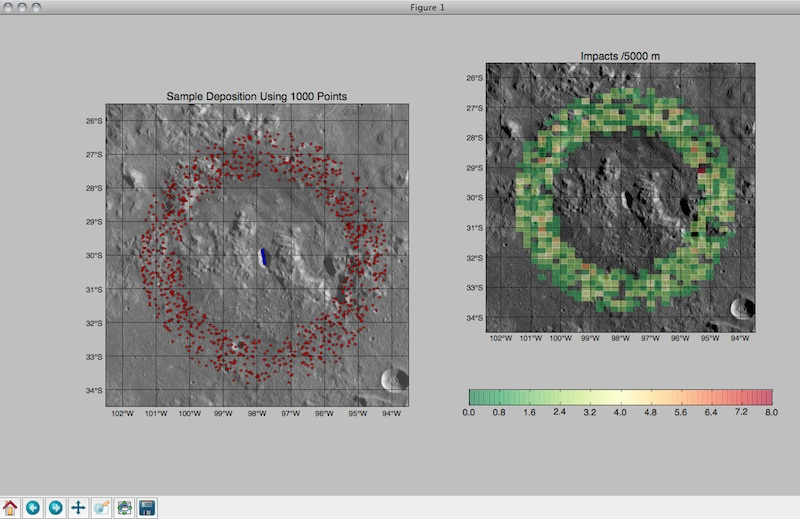
\includegraphics{sample.jpg}

This model seeks to provide a visualization of a strombolian ejection on the lunar surface.  These are relatively simple models that do not account for the type of ejected material and need not account for atmosphere.


\chapter{Installing the Strombolian Volcano Simulator}
\label{Installation:installation}\label{Installation:installing-the-strombolian-volcano-simulator}\label{Installation:welcome-to-strombolian-eruption-simulation-documentation}\label{Installation::doc}

\section{SVS Dependencies}
\label{Installation:svs-dependencies}
SVS requires Python and depends on several other freely available Python
modules. Prior to installing SVS, you should make sure its dependencies are met.


\begin{threeparttable}
\capstart\caption{SVS Dependencies}

\begin{tabulary}{\linewidth}{|L|L|}
\hline
\textbf{
Dependency
} & \textbf{
Requirement
}\\\hline

\href{http://www.python.org}{Python 2.7+}
 & 
Required
\\\hline

\href{http://numpy.scipy.org/}{NumPy}
 & 
Required
\\\hline

\href{http://gdal.org/}{GDAL}
 & 
Required
\\\hline

\href{http://pypi.python.org/pypi/GDAL/}{GDAL Python Bindings}
 & 
Required
\\\hline

\href{http://matplotlib.org/users/installing.html}{Matplotlib}
 & 
Required
\\\hline

\href{https://developers.google.com/appengine/docs/python/images/installingPIL}{Python Imaging Library}
 & 
Required
\\\hline

\href{http://matplotlib.org/basemap/users/installing.html}{Basemap}
 & 
Required
\\\hline
\end{tabulary}

\end{threeparttable}


Note that SVS is not tested with Python 3.x.


\section{Installing}
\label{Installation:installing}
SVS is distributed as a stand alone script and therefore does not require installation.  This documentation is distributed locally, with SVS.  Simply place the script in a convenient directory.

Note that SVS does have a number of dependencies.  These facilitate data processing, shapefile output generation, and topographic profile extraction.  They are required and should therefore be installed prior to attempting to run SVS.


\subsection{Installation on OS X}
\label{Installation:installation-on-os-x}

\subsubsection{Python}
\label{Installation:python}\begin{quote}

Python ships with Mac OS X.  It is not necessary to install a different version.  Should you wish to, numerous online tutorials cover the installation of an additional python installation.  As of 10.6 (possibly earlier) the default Python installation should be 64bit.
\end{quote}


\subsubsection{Numpy}
\label{Installation:id1}\begin{quote}

Numerical Python is available for OS X via either pip or easy\_install:

\begin{Verbatim}[commandchars=\\\{\}]
\$ easy\_install numpy
\$ pip install numpy
\end{Verbatim}
\end{quote}


\subsubsection{NumPy, PIL, MatPlotLib}
\label{Installation:numpy-pil-matplotlib}\begin{quote}

Alternatively, you can install NumPy, along with PIL and Matplotlib via binaries.  These are compiled and made available by KyngChaos via his

\href{http://www.kyngchaos.com/software/python}{OS X GIS Ports}

Simply download the binares and install them.  While you are there, you might grab SciPy, it will be useful sometime soon on some other project!
\end{quote}


\subsubsection{GDAL \& GDAL Python Bindings}
\label{Installation:gdal-gdal-python-bindings}\begin{quote}

If you are using a package manager (Fink, MacPorts, Homebrew) install GDAL and the python bindings via that.  Otherwise, KyngChaos provides precompiled binaries for installation.

\href{http://www.kyngchaos.com/software/frameworks}{GDAL Complete}
\end{quote}


\subsubsection{Basemap}
\label{Installation:id2}\begin{quote}

This is slightly more complex and an OS X DMG will be forth coming.  The simplest methods, installation via automated source compilation is documented by the \href{https://modelingguru.nasa.gov/docs/DOC-1847}{NASA Modelling Guru}.  In short, if you have macports, fink, or homebrew installed you can utilize one of the following, respectively.  Otherwise, you are going to need to build via source...:

\begin{Verbatim}[commandchars=\\\{\}]
\$ fink install matplotlib
\$ port install py-matplotlib-basemap
\$ brew install basemap
\end{Verbatim}
\end{quote}


\subsection{Installation on Windows}
\label{Installation:installation-on-windows}
Windows installation


\subsubsection{NumPy, PIL, Basemap, Matplotlib, GDAL Python Bindings}
\label{Installation:numpy-pil-basemap-matplotlib-gdal-python-bindings}\begin{quote}

Christopher Gohlke has made a large number of binaries available for windows users.  All dependencies save the core GDAL libraries can be installed via his site.

\href{http://www.lfd.uci.edu/~gohlke/pythonlibs/}{Windows Python Packages}
\end{quote}

\begin{notice}{warning}{Warning:}
Install the GDAL core package before installing the gdal python bindings.
\end{notice}


\subsubsection{GDAL Core}
\label{Installation:gdal-core}\begin{quote}

Installation of GDAL Core is slightly more complex.  First, download the binary package from \href{http://www.gisinternals.com/sdk/PackageList.aspx?file=release-1600-gdal-1-9-2-mapserver-6-2-0.zip}{GIS Internals}.  This is gdal-\#\#-\#\#\#\#-core.msi.  If you are an ArcGIS user, you likely want the MSVC 2008 version.  Install this package as you normally would.

Two tutorials will be of assistance in getting GDAL setup in your PATH.  Either tutorial covers the installation process.
\begin{enumerate}
\item {} 
\href{http://php.scripts.psu.edu/jzl5325/wordpress/?p=60}{My tutorial will exist as long as my Penn State account stays active}

\item {} 
This \href{http://www.gis.usu.edu/~chrisg/python/2009/docs/gdal\_win.pdf}{USU tutorial} also covers installation as a pdf.

\end{enumerate}
\end{quote}


\subsection{Installation on Linux}
\label{Installation:installation-on-linux}\begin{quote}

The simplest installation for users who are likely comfortable with more complex installations!:

\begin{Verbatim}[commandchars=\\\{\}]
\$ sudo apt-get install python-pip
\$ sudo apt-get install gdal-bin python-gdal
\$ pip install matplotlib
\$ pip install numpy
\$ pip install basemap
\end{Verbatim}
\end{quote}

\begin{notice}{note}{Note:}
If for some strange reason python is not already installed, you will be asked to install python running the first command, above.
\end{notice}


\chapter{Using SVS}
\label{Using:using-svs}\label{Using:using}\label{Using::doc}
This page documents the implementation and usage of SVS.  The model is constantly evolving and the documentation may not cover all pertinent features.  See the doc strings in the code as these are the most up to date indication of functionality.  We are current as of 0.1.


\section{Usage}
\label{Using:usage}
The basic usage of the script displays the iterative deposition of particles in a matplotlib gui window.  After the deposition has completed it is possible to save the window to a PNG.

Two plots are displayed, the first is a movie that tracks where particles are deposited.  The second, populated at the completion of deposition, is a density map, showing points per grid cell.


\subsection{Running the iterative deposition}
\label{Using:running-the-iterative-deposition}
To get help, and see available parameters:

\begin{Verbatim}[commandchars=\\\{\}]
\$ python simulation2.py --help
\end{Verbatim}

To run a basic model with all default ejection parameters:

\begin{Verbatim}[commandchars=\\\{\}]
\$ python simulation2.py
\end{Verbatim}

\begin{notice}{note}{Note:}
The default model emplaces 500 points with ejection velocity between 300 and 325m/s and ejection angle between 30 and 60 degrees.  Azimuth of ejection is random.
\end{notice}

To provide a fixed ejection angle:

\begin{Verbatim}[commandchars=\\\{\}]
\$ python simulation2.py --angle 45
\$ python simulation2.py -a 45
\end{Verbatim}

To provide your own range of ejection angles:

\begin{Verbatim}[commandchars=\\\{\}]
\$ python simulation2.py --angle minAngle maxAngle
\$ python simulation2.py --angle 25 75
\end{Verbatim}

To provide your fixed ejection velocity:

\begin{Verbatim}[commandchars=\\\{\}]
\$ python simulation2.py --velocity 400
\$ python simulation2.py -v 400
\end{Verbatim}

To provide a range of velocities:

\begin{Verbatim}[commandchars=\\\{\}]
\$ python simulation2.py -v 350 425
\$ python simulation2.py --velocity 275 450
\end{Verbatim}


\subsection{Altering the grid size}
\label{Using:altering-the-grid-size}
By default, the model utilizes a 1000m\textasciicircum{}2 grid cell to track deposition density.  The color bar indicating deposition scales with the data.  To alter the grid cell size you can define Pixel Per Grid Cell as :math:: x * 100m, where x is some scalar multiplier.  For example, when $x = 10$, grid size is $1000m^2$.  When $x = 50$, grid size is $5000m^2$.  This can be altered using:

\begin{Verbatim}[commandchars=\\\{\}]
\$ python simulation2.py --ppg 50
\end{Verbatim}


\subsection{Writing to a shapefile}
\label{Using:writing-to-a-shapefile}
Users can write the resulting model to a shapefile using the following:

\begin{Verbatim}[commandchars=\\\{\}]
\$ python simulation2.py --shapefile SOMENAME.shp
\end{Verbatim}

\begin{notice}{note}{Note:}
The resulting file is `timestamped' with an iteration number.  It is therefore possible, as of ArcGIS 10.0 to utilize the time slider to explore the temporality of deposition.  We suggest setting the time specification to years when using this type of visualization.
\end{notice}


\subsection{Combining Arguments}
\label{Using:combining-arguments}
Combining arguments is completely valid,for example the following would define a custom ejection angle, velocity, and output the results to a shapefile.:

\begin{Verbatim}[commandchars=\\\{\}]
\$ python simulation2.py -a 35 80 -v 375 425 --shapefile MyTestRun.shp
\end{Verbatim}


\subsection{Speed}
\label{Using:speed}
Iterative deposition in a live matplotlib windows is suitably fast for low number of \emph{n}.  When \emph{n} \textgreater{} 10,000 we suggest using the \emph{--fast} flag.  This flag bypasses the interactive visualization and writes directly to a shapefile.  In this way, it is no longer possible to visualize the results in matplotlib.  The \emph{--fast} implementation is multicore enabled and will utilize all available processing capability on your machine.:

\begin{Verbatim}[commandchars=\\\{\}]
\$ python simulation2.py --fast MyFastShapefile.shp
\end{Verbatim}

\begin{notice}{warning}{Warning:}
It is possible that python will warn you that your output is not a directory.  This is because a shapefile with the same name already exists in the directory.  Either change the name of your output or delete the old output.
\end{notice}


\section{Location}
\label{Using:location}
Currently this model is focused around the dark ring material eruption (Mare Orientale).  The underlying basemap is hardcoded as is the output shapefile.  With relatively trivial alteration to the code, it will be possible to extend the model.


\section{Ejection Model}
\label{Using:ejection-model}
We are modeling this ejection using the most basic, atmosphere free, trajectory model.  Briefly, here are the steps we take to calculate the position of the deposited material.
\begin{enumerate}
\item {} 
Randomly determine the ejection angle, $\theta$

\item {} 
Calculate $\theta^2$

\item {} 
Randomly determine velocity from the given range, $v$

\item {} 
Compute $v^2$

\item {} 
Compute total possible theoretical distance:
\begin{quote}

distance = $(v^2 * \theta)/g$, where $g = 1.62m/s$
\end{quote}

\item {} 
Randomly determine some ejection azimuth between 0 and 360.

\end{enumerate}

Next we calculate the idealized height of the projectile over the body at 100m intervals.  This interval was selected as it is the nominal resolution of the WAC DTM.  We therefore know: total theoretical travel distance,  azimuth, height above a planar surface at 100m interval.  Using this information we then convert from geographic coordinates to pixel space and:
\begin{quote}
\begin{enumerate}
\item {} 
Extract the underlying topography along the line of travel.  This is stored as an nx1 array of elevation data.

\begin{notice}{note}{Note:}
We are using a nearest neighbor interpolation.  It is possible that the line of travel `clips' the corner of a pixel.  We are utilizing the spot elevation at that pixel in our calculation.  This \emph{should} be relatively safe due to Tobler's first law and the resolution of our data.
\end{notice}

\item {} 
Normalize the trajectory elevation to the elevation of the ejection point.  To do this we are subtracting the elevation at ejection from each index of the trajectory vector.

\item {} 
Add the absolute value of the elevation vector to the the elevation vector.  Here the goal is to have all values $>=$ 0.  This allows for the vectorized computation of elements and is done to speed program computation.

\item {} 
Subtract the elevation vector from the trajectory vector to calculate the distance above our modified topography.

\item {} 
Add the negative offset to the elevation back to the newly generated `distance above the topographic surface' raster.

\end{enumerate}
\begin{quote}

\begin{notice}{note}{Note:}
This will need to be modified to test for sign should the ejection point be higher than 0m.
\end{notice}
\end{quote}
\begin{enumerate}
\setcounter{enumi}{5}
\item {} 
Return the index of impact point $* 100$.  This is the total distance in meters that the projectile travelled in pixel space and an estimation (within 99m) of total travel distance.

\end{enumerate}
\end{quote}



\renewcommand{\indexname}{Index}
\printindex
\end{document}
